\documentclass[]{book}
\usepackage{lmodern}
\usepackage{amssymb,amsmath}
\usepackage{ifxetex,ifluatex}
\usepackage{fixltx2e} % provides \textsubscript
\ifnum 0\ifxetex 1\fi\ifluatex 1\fi=0 % if pdftex
  \usepackage[T1]{fontenc}
  \usepackage[utf8]{inputenc}
\else % if luatex or xelatex
  \ifxetex
    \usepackage{mathspec}
  \else
    \usepackage{fontspec}
  \fi
  \defaultfontfeatures{Ligatures=TeX,Scale=MatchLowercase}
\fi
% use upquote if available, for straight quotes in verbatim environments
\IfFileExists{upquote.sty}{\usepackage{upquote}}{}
% use microtype if available
\IfFileExists{microtype.sty}{%
\usepackage{microtype}
\UseMicrotypeSet[protrusion]{basicmath} % disable protrusion for tt fonts
}{}
\usepackage{hyperref}
\hypersetup{unicode=true,
            pdftitle={Olimpiadinės biologijos gidas},
            pdfauthor={Paulius Alaburda},
            pdfborder={0 0 0},
            breaklinks=true}
\urlstyle{same}  % don't use monospace font for urls
\usepackage{natbib}
\bibliographystyle{apalike}
\usepackage{longtable,booktabs}
\usepackage{graphicx,grffile}
\makeatletter
\def\maxwidth{\ifdim\Gin@nat@width>\linewidth\linewidth\else\Gin@nat@width\fi}
\def\maxheight{\ifdim\Gin@nat@height>\textheight\textheight\else\Gin@nat@height\fi}
\makeatother
% Scale images if necessary, so that they will not overflow the page
% margins by default, and it is still possible to overwrite the defaults
% using explicit options in \includegraphics[width, height, ...]{}
\setkeys{Gin}{width=\maxwidth,height=\maxheight,keepaspectratio}
\IfFileExists{parskip.sty}{%
\usepackage{parskip}
}{% else
\setlength{\parindent}{0pt}
\setlength{\parskip}{6pt plus 2pt minus 1pt}
}
\setlength{\emergencystretch}{3em}  % prevent overfull lines
\providecommand{\tightlist}{%
  \setlength{\itemsep}{0pt}\setlength{\parskip}{0pt}}
\setcounter{secnumdepth}{5}
% Redefines (sub)paragraphs to behave more like sections
\ifx\paragraph\undefined\else
\let\oldparagraph\paragraph
\renewcommand{\paragraph}[1]{\oldparagraph{#1}\mbox{}}
\fi
\ifx\subparagraph\undefined\else
\let\oldsubparagraph\subparagraph
\renewcommand{\subparagraph}[1]{\oldsubparagraph{#1}\mbox{}}
\fi

%%% Use protect on footnotes to avoid problems with footnotes in titles
\let\rmarkdownfootnote\footnote%
\def\footnote{\protect\rmarkdownfootnote}

%%% Change title format to be more compact
\usepackage{titling}

% Create subtitle command for use in maketitle
\providecommand{\subtitle}[1]{
  \posttitle{
    \begin{center}\large#1\end{center}
    }
}

\setlength{\droptitle}{-2em}

  \title{Olimpiadinės biologijos gidas}
    \pretitle{\vspace{\droptitle}\centering\huge}
  \posttitle{\par}
    \author{Paulius Alaburda}
    \preauthor{\centering\large\emph}
  \postauthor{\par}
      \predate{\centering\large\emph}
  \postdate{\par}
    \date{2019-11-23}

\usepackage{booktabs}

\begin{document}
\maketitle

{
\setcounter{tocdepth}{1}
\tableofcontents
}
\hypertarget{izanga}{%
\chapter{Įžanga}\label{izanga}}

Knyga yra nuolatos atnaujinama. Tai nėra galutinis produktas. Laukite naujienų!

\hypertarget{turinys}{%
\section{Turinys}\label{turinys}}

\begin{itemize}
\tightlist
\item
  Augalai

  \begin{itemize}
  \tightlist
  \item
    Augalų struktūra ir augimas
  \item
    Medžiagų pernaša augaluose
  \item
    Augalų dauginimasis
  \item
    Augalų hormonai
  \end{itemize}
\item
  Ląstelės biologija

  \begin{itemize}
  \tightlist
  \item
    Mikroskopija
  \item
    Ląstelės struktūra
  \item
    Ląstelės funkcijos
  \item
    Funkcinis ir struktūrinis ląstelių santykis
  \item
    Ląstelės membrana
  \item
    Ląstelės metabolizmas
  \end{itemize}
\item
  Biochemija

  \begin{itemize}
  \tightlist
  \item
    Fermentų kenetika
  \item
    Makromolekulės
  \end{itemize}
\item
  Gyvūnai
\item
  Bakterijos
\item
  Grybai
\item
  Archėjos
\item
  Pirmuonys
\end{itemize}

\hypertarget{augalai}{%
\chapter{Augalai}\label{augalai}}

\hypertarget{izanga-1}{%
\section{Įžanga}\label{izanga-1}}

Augalai buvo mano nemėgstamiausia tema ruošiantis olimpiadoms, bet dabar manau visiškai priešingai. Augalai yra itin svarbūs mums - dėl bulvių maro Airijoje mirė penktadalis gyventojų, EUropoje įvyko ekonominė krizė dėl tulpių gumbų, o šafranas - žiedo piestelės - yra brangiausias prieskonis pasaulyje. Jeigu ne grūdai, ko gero nebūtume turėję feodalizmo ir nebūtume tyrinėję genetikos! Pažindamas augalus gali pažinti ne tik savo mitybą, bet ir žmogaus istoriją.

\hypertarget{lastele}{%
\section{Ląstelė}\label{lastele}}

Skiriasi nuo eukariotinės gyvūno ląstelės šiais bruožais:

\begin{enumerate}
\def\labelenumi{\arabic{enumi}.}
\tightlist
\item
  Chloroplastai - išsidėsto ląstelės kraštuose, vykdo fotosintezę
\item
  Centrinė vakuolė - viena, yra ląstelės centre, palaiko ląstelės formą, reguliuoja ląstelės vidinę terpę
\item
  Plazmodezmos - tai citoplazminis tiltelis tarp dviejų augalo ląstelių. Per jį gali judėti citoplazmos turinys, organelės bei virusai.
\item
  Ląstelės sienelė - ekstraląstelinė (\emph{extra} - išorėje) struktūra, apsaugo nuo sužeidimų, palaiko formą, riboja vandens patekimą į ląstelę\\
\item
  NĖRA centriolių - augalų ląstelės nevykdo citokinezės, iš Goldžio aparato pūslelių formuojasi membrana tarp dukterinių ląstelių
\end{enumerate}

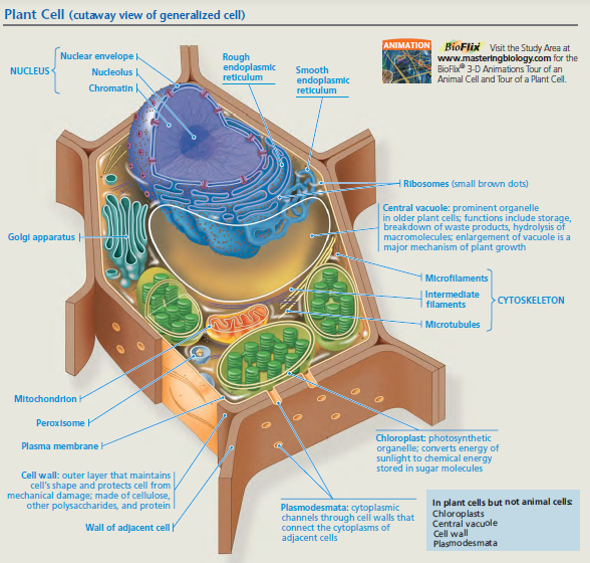
\includegraphics[width=500px]{static/augalai/plant_cell}

\hypertarget{chloroplastai-ir-fotosinteze}{%
\section{Chloroplastai ir fotosintezė}\label{chloroplastai-ir-fotosinteze}}

Chloroplastai turi dvigubą membraną (pūslelė pūslelėje), viduje yra stroma, kurioje yra išsidėstę tilakoidai. Tilakoiduose yra fotosintezės aparatas, tilakoidai yra išsidėstę į granas. Šviesos ir tamsos reakcijos vyksta chloroplaste - šviesos reakcijos vyksta tilakoidų membranoje (protonų gradientas ATP sintezei kaupiamas tilakoidų viduje), tamsos reakcijos vyksta chloroplasto stromoje.

Fotosintezę vykdo ne tik augalai, bet ir protistai (\emph{euglena}) bei prokariotai (\emph{cianobakterijos}, vietoje chloroplastų turi tilakoidus citoplazmoje). Fotosintezė yra autotrofų mitybos būdas - jie pasigamina organines medžiagas iš CO2 ir kitų neorganinių medžiagų. Autotrofai yra biosferos gamintojai ir taip pat suteikia organines medžiagas likusiems organizmams - vartotojams (heterotrofams).

Fotosintezė vyksta chloroplastuose ir yra sudaryta iš dviejų stadijų:

\begin{enumerate}
\def\labelenumi{\arabic{enumi}.}
\tightlist
\item
  Šviesos fazės - šviesa panaudojama aktyvinti vandens elektronus ir jais redukuoti NADP iki NADPH ir protonų gradientu sintetinti ATP iš ADP ir fosfato grupės.
\item
  Tamsos fazės - ATP ir NADPH yra naudojama kaip energijos šaltinis CO2 fiksacijai. Galutinis produktas - organiniai angliavandeniai, dažniausiai gliukozė ir fruktozė.
\end{enumerate}

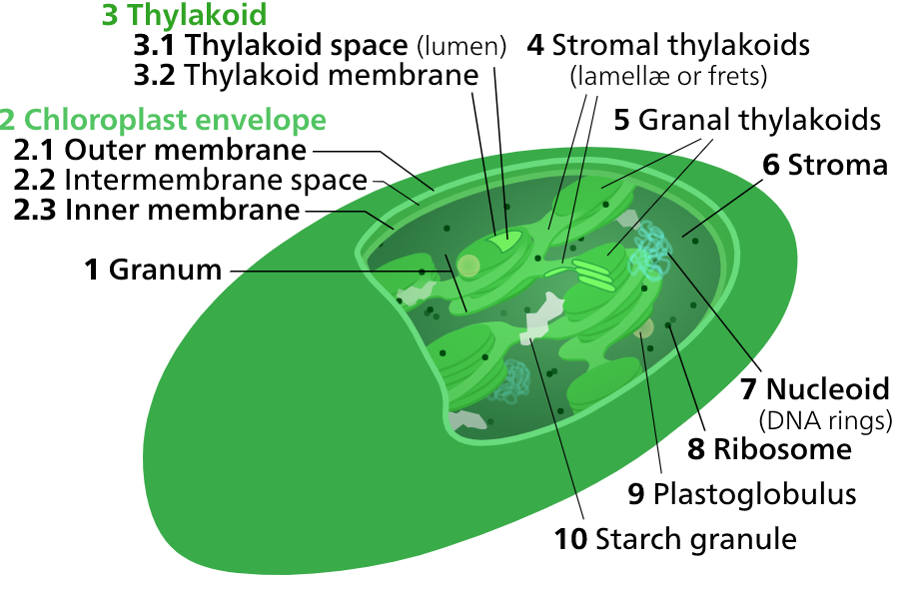
\includegraphics[width=500px]{static/augalai/chloroplast}
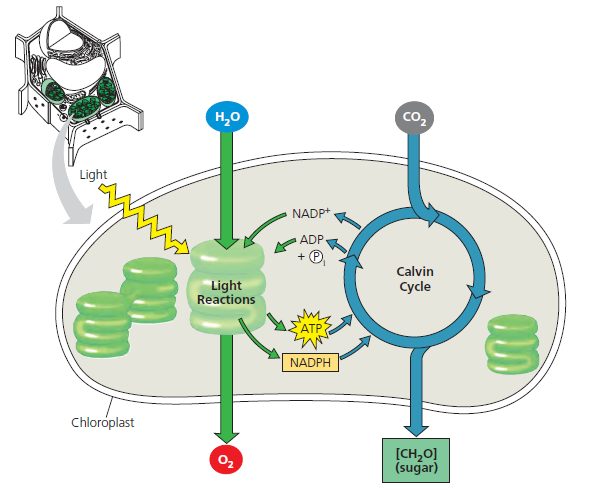
\includegraphics[width=500px]{static/augalai/photosynthesis}

\hypertarget{plazmodezmos}{%
\section{Plazmodezmos}\label{plazmodezmos}}

Augalinės ląstelės tarpusavyje turi plazminės membranos vamzdelius, kurie susisiekia per ląstelės sienelę. Stambios, pro jas gali judėti organelės, vanduo, makromolekulės. Greitesnė medžiagų pernaša, signalas tarp ląstelių perduodamas toliau. Bet gali judėti ir viruso DNR/RNR (tabako virusas), grybų hifai, bakterijos.

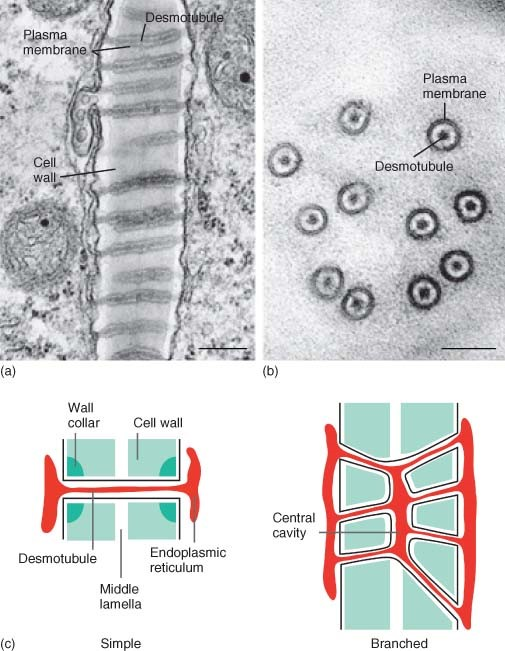
\includegraphics[width=500px]{static/augalai/plasmodesmata}

\hypertarget{lasteles-sienele}{%
\section{Ląstelės sienelė}\label{lasteles-sienele}}

Augalo ląstelės sienelė sudaryta iš trijų pagrindinių dalių - celiuliozės, pektino ir hemiceliuliozės. Hemiceliuliozė tarpusavyje apjungia skirtingus celiuliozės pluoštus, o pektinas suteikia audiniui standumo ir apjungia ląsteles tarpusavyje.

Augalo ląstelė visada turi pirminę sienelę, bet taip pat gali turėti ir antrinę sienelę, kuri yra įprastai storesnė, turi lignino bei suberino ir suteikia audiniui tvirtumo.

Pagal sienelės išsivystymą galima išskirti tris ląstelės sienelės tipus:

\begin{enumerate}
\def\labelenumi{\arabic{enumi}.}
\tightlist
\item
  Parenchimą -- minkštieji audiniai
\item
  Kolenchimą -- augančios dalys
\item
  Sklerenchimą -- nedalyvauja fotosintezėje, atraminė funkcija
\end{enumerate}

\hypertarget{plastides}{%
\section{Plastidės}\label{plastides}}

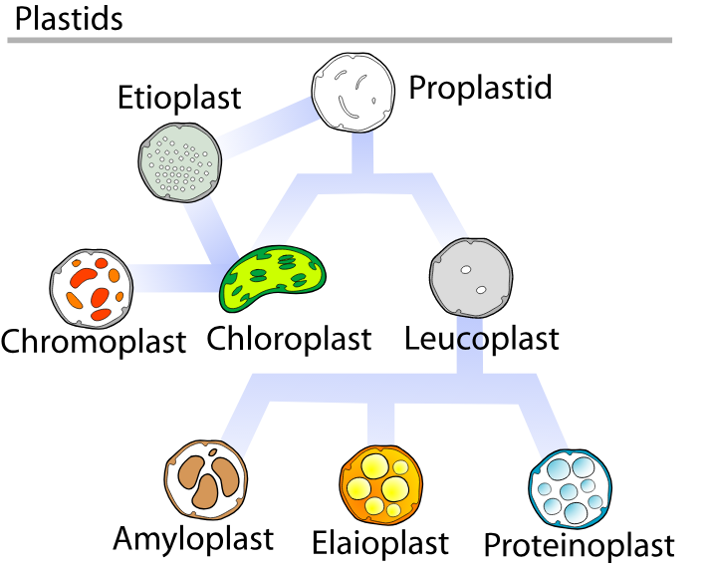
\includegraphics[width=500px]{static/augalai/plastids}

Chloroplastas yra plastidė, tačiau plastidės gali specializuotis atlikti kitas funkcijas (dažniausiai, kaupti specifines medžiagas).

Proplastidė - nediferencijuota plastidė
Chromoplastas - kaupia pigmentus
Amiloplastas - kaupia angliavandenius
Elajoplastas - kaupia riebalines medžiagas
Proteinoplastas - kaupia baltymus

\hypertarget{centrine-vakuole}{%
\section{Centrinė vakuolė}\label{centrine-vakuole}}

\begin{enumerate}
\def\labelenumi{\arabic{enumi}.}
\tightlist
\item
  Kaupia medžiagas
\item
  Kaupia druskų perteklių, nuodingas medžiagas, apykaitos produktai
\item
  Lizosominė funkcija
\item
  Elektrocheminis gradientas
\item
  Turgoras
\item
  Ląstelių augimas
\end{enumerate}

\hypertarget{augalo-daliu-adaptacijos}{%
\section{Augalo dalių adaptacijos}\label{augalo-daliu-adaptacijos}}

\hypertarget{stiebu-adaptacijos}{%
\subsection{Stiebų adaptacijos}\label{stiebu-adaptacijos}}

\begin{enumerate}
\def\labelenumi{\arabic{enumi}.}
\tightlist
\item
  Rizomai -- horizontalus stiebas po žeme (vilkdalgis)
\item
  Svogūnai -- stiebo sustorėjimas po žeme su maisto medžiagas kaupiančiais lapais (svogūnai, tulpės)
\item
  Ūsai -- stiebo išaugos, kurios leidžia nelytiškai daugintis (braškės)
\item
  Stiebagumbiai -- požeminis stiebas, turintis pumpurus (bulvė)
\end{enumerate}

\hypertarget{saknu-adaptacijos}{%
\subsection{Šaknų adaptacijos}\label{saknu-adaptacijos}}

\begin{enumerate}
\def\labelenumi{\arabic{enumi}.}
\tightlist
\item
  Šakniavaisiai -- atlieka kaupiamąją funkciją (burokėlis)
\item
  Pneumatoforai -- išdygsta į orą, kai pelkėse nėra deguonies (mangrovė)
\item
  Atraminės šaknys -- kai dirva minkšta, padeda augalui išsilaikyti (banjanas)
\item
  Orinės šaknys -- dygsta ore, įsiskerbusios įsišaknyja (monstera)
\end{enumerate}

\hypertarget{lapu-adaptacijos}{%
\subsection{Lapų adaptacijos}\label{lapu-adaptacijos}}

\begin{enumerate}
\def\labelenumi{\arabic{enumi}.}
\tightlist
\item
  Ūsai (ang. tendrils) -- padeda prisitvirtinti prie paviršių (vijokliniai augalai, pupa)
\item
  Spygliai -- taip, kaktuso „lapas`` yra stiebas
\item
  Kaupia maisto medžiagas -- visi sukulentai
\item
  Dauginimosi lapai -- išdygę nukrenta ir sudygsta ant žemės
\item
  Pažiedlapiai -- vainiklapių pamaina (puansentija)
\end{enumerate}

\hypertarget{iliustracijos}{%
\section{Iliustracijos}\label{iliustracijos}}

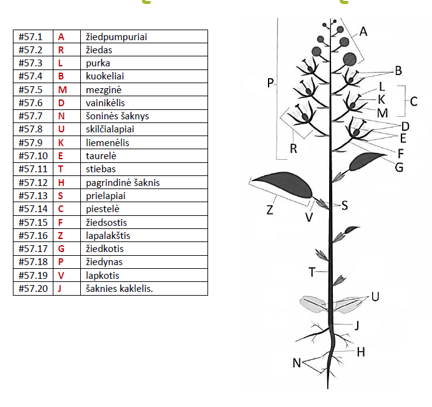
\includegraphics[width=500px]{static/augalai/augalo_dalys}
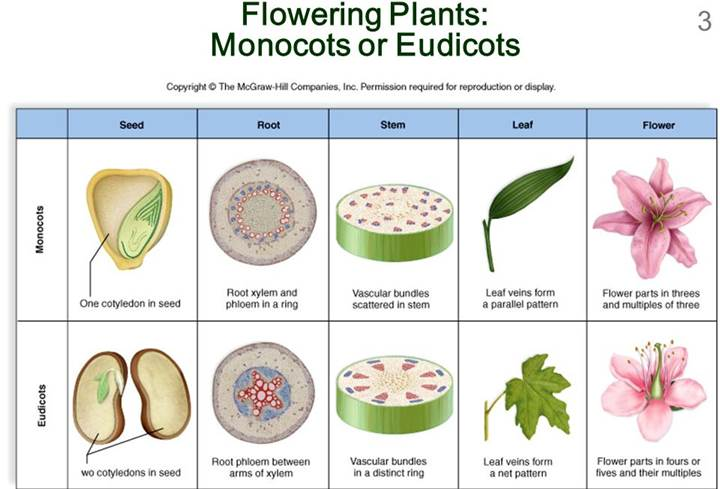
\includegraphics[width=500px]{static/augalai/dvi_vienskilciai}
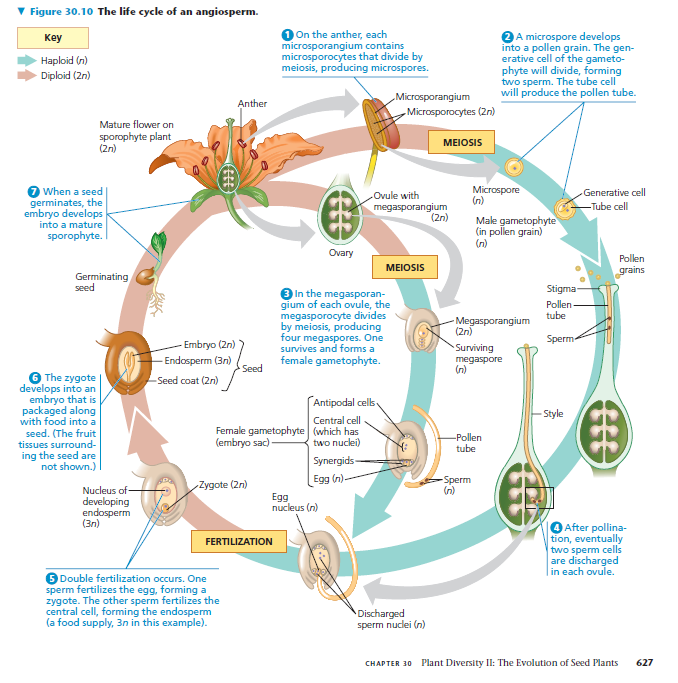
\includegraphics[width=500px]{static/augalai/gaubtasekliai}
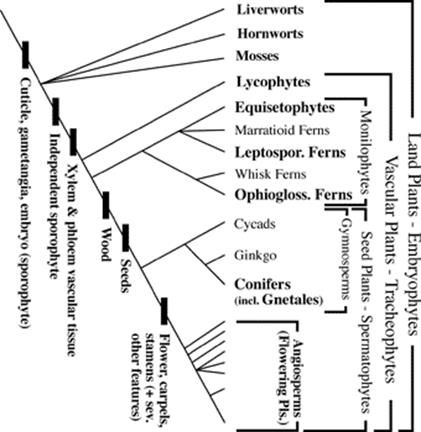
\includegraphics[width=500px]{static/augalai/klasifikacija}
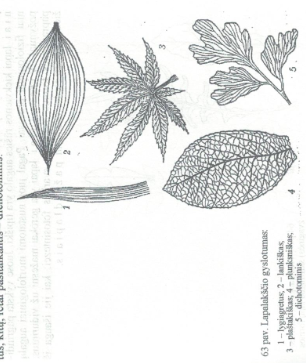
\includegraphics[width=500px]{static/augalai/lapo_gyslotumas}
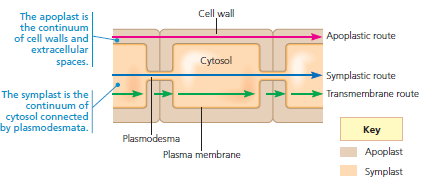
\includegraphics[width=500px]{static/augalai/medz_judejimas}
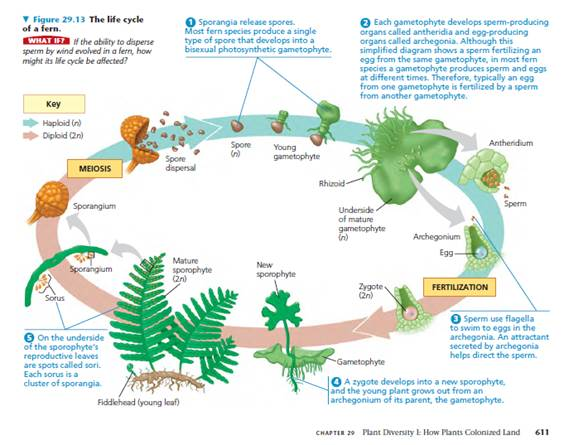
\includegraphics[width=500px]{static/augalai/papartunai}
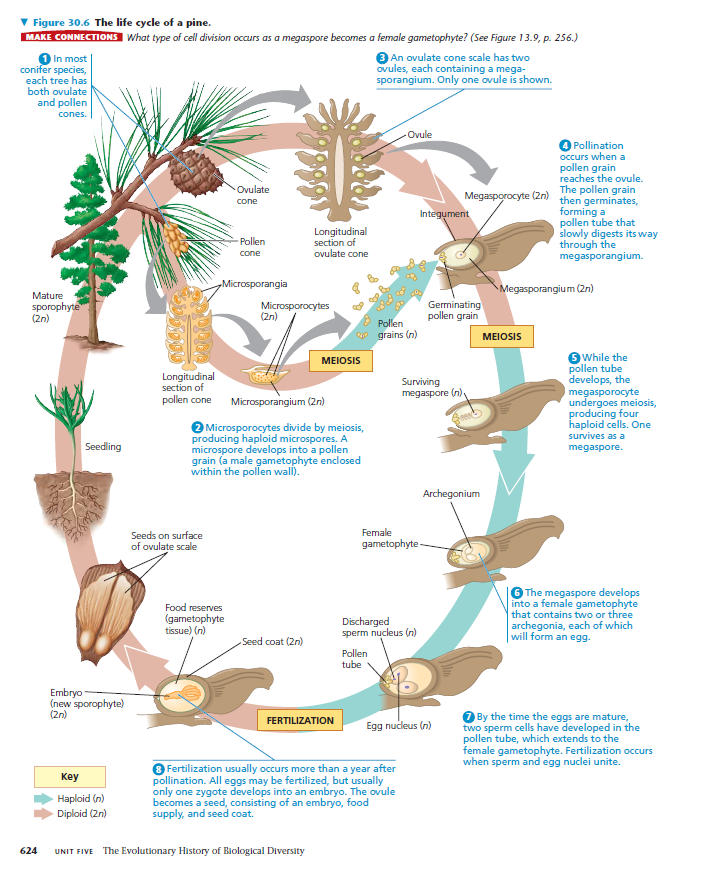
\includegraphics[width=500px]{static/augalai/plikasekliai}
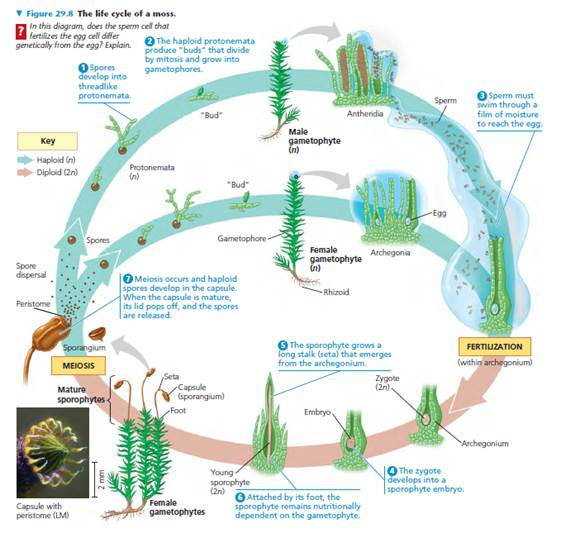
\includegraphics[width=500px]{static/augalai/samanunai}
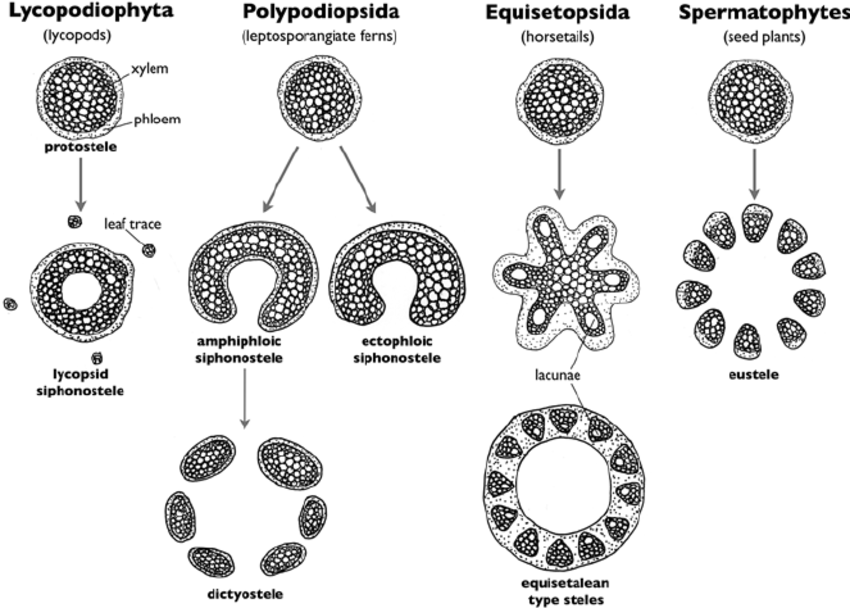
\includegraphics[width=500px]{static/augalai/steles_1}
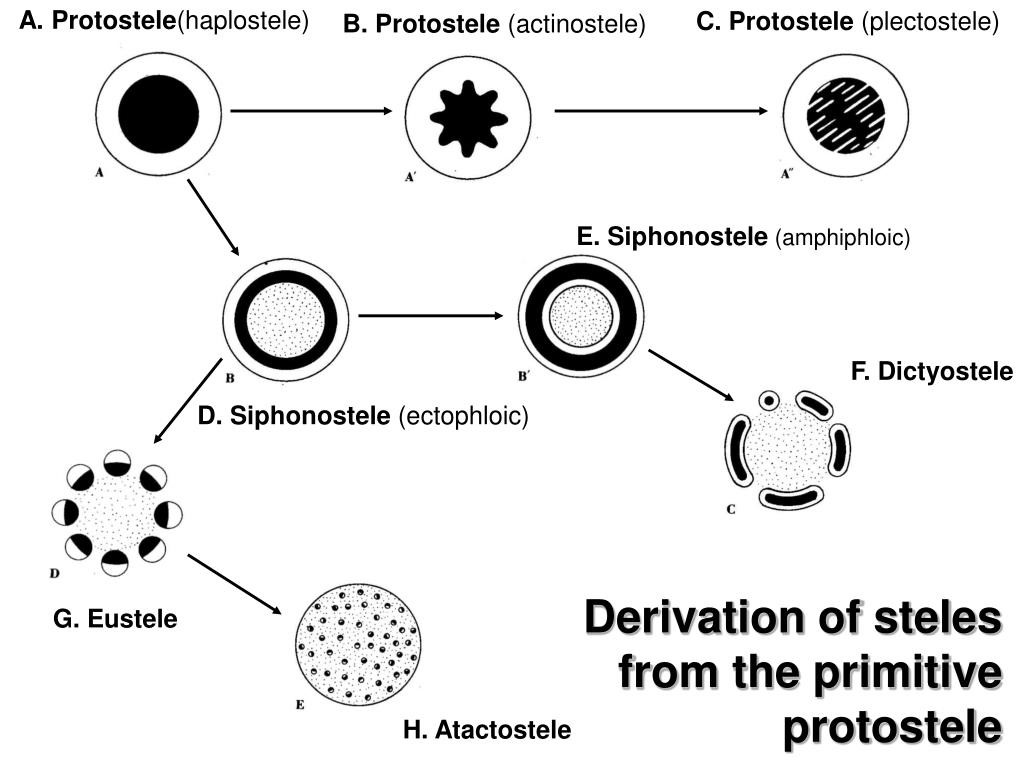
\includegraphics[width=500px]{static/augalai/steles_2}
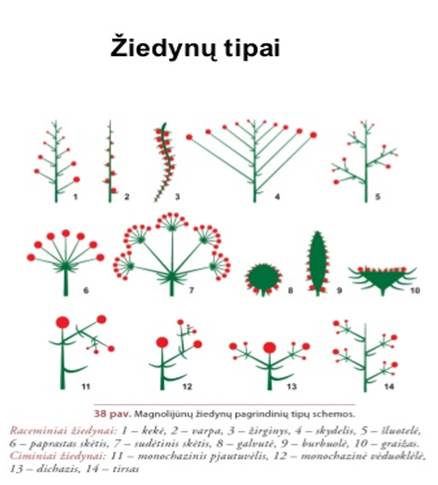
\includegraphics[width=500px]{static/augalai/ziedynu_tipai}

\bibliography{book.bib,packages.bib}


\end{document}
